%%% Intro.tex --- 
%% 
%% Filename: Intro.tex
%% Description: 
%% Author: Ola Leifler
%% Maintainer: 
%% Created: Thu Oct 14 12:54:47 2010 (CEST)
%% Version: $Id$
%% Version: 
%% Last-Updated: Thu May 19 14:12:31 2016 (+0200)
%%           By: Ola Leifler
%%     Update #: 5
%% URL: 
%% Keywords: 
%% Compatibility: 
%% 
%%%%%%%%%%%%%%%%%%%%%%%%%%%%%%%%%%%%%%%%%%%%%%%%%%%%%%%%%%%%%%%%%%%%%%
%% 
%%% Commentary: 
%% 
%% 
%% 
%%%%%%%%%%%%%%%%%%%%%%%%%%%%%%%%%%%%%%%%%%%%%%%%%%%%%%%%%%%%%%%%%%%%%%
%% 
%%% Change log:
%% 
%% 
%% RCS $Log$
%%%%%%%%%%%%%%%%%%%%%%%%%%%%%%%%%%%%%%%%%%%%%%%%%%%%%%%%%%%%%%%%%%%%%%
%% 
%%% Code:


\chapter{TLM-Based Co-Modeling Editor and Co-Simulation Framework}
\label{cha:tlm}


This chapter is based on the following paper:

\begin{itemize}
	
	
	\item  \textbf{Alachew Mengist}, Adeel Asghar, Adrian Pop, Peter Fritzson, Willi Braun, Alexander Siemers and Dag Fritzson.\textbf{ An Open-Source Graphical Composite Modeling Editor and Simulation Tool Based on FMI and TLM Co-Simulation.} In Proceedings of the 11th International Modelica Conference, Versailles, France, September 21-23, 2015. 
	
\end{itemize}

\section{Introduction}
\label{sec:tlmintroduction}

Industrial products often consist of many components which have been developed by different suppliers
using different modeling and simulation tools. An integrated modeling and simulation support is needed in order to
integrate all the parts of a complex product model. TLM-based modeling and co-simulation is an important technique for
modeling, connecting, and simulation of especially mechanical systems, which is simple, numerically stable, and efficient.
A number of tool specific simulation models, such as Modelica models, SimuLink models, Adams models, BEAST models, etc., 
have successfully been connected and simulated using TLM-based co-simulation.

This has successfully been demonstrated by integrating and connecting several different simulation
models, especially for mechanical applications. Such an integrated model consisting of several model parts
is here called a composite model since it is composed of several sub-models. Another name used for such a
model is meta-model, since it is a model of models. In earlier work \cite{tlmalexander05,tlmsiemers06}, Modelica with its object oriented modeling capabilities and its standardized graphical notations has demonstrated the possibilities for meta-modeling/composite modeling of
mechanical systems using TLM.

The availability of a general XML-based composite modeling language \cite{tlmalexander05} is an
important aspect of our TLM-based modeling and co-simulation framework. However, modelers
developing composite models are likely to take advantage of the additional availability of tools that
assist them with respect to the composite modeling process (i.e., the process of creating and/or editing a
composite model, here represented and stored as XML). 

We introduce a graphical composite model editor which is an extension and specialization of the
OpenModelica connection editor OMEdit. In the context of this work a composite
model is composed of several sub-models including the interconnections between these sub-models. 
The editor supports creating, viewing and editing a composite model both in textual and graphical representation. 
The system supports simulation of composite models consisting of sub-models created using different tools.. It is also integrated
with the SKF TLM-based cosimulation framework.

\section{TLM-Based Co-simulation Framework}
\label{sec:tlmframework}

As men\-tioned, a gen\-eral frame\-work for com\-pos\-ite model-based co-simulation has pre\-vi\-ously 
been de\-signed and im\-ple\-mented in  \cite{tlmalexander05}. The design goals for the simulation part of that framework
were portability, simplicity to incorporate additional simulation tools, and computational efficiency. 
It is also the framework used for \acrshort{tlm}-based composite model co-simulation described in this chapter.
The TLM composite model co-simulation is primarily handled by the central simulation engine of the framework 
called the \acrshort{tlm} simulation manager. It is a stand-alone program that reads an \acrshort{xml} definition
of the coupled simulation as defined in \cite{tlmalexander05}. It then starts external model simulations and
provides the communication bridge between the running simulations using the TLM \cite{tlmlakov06} method. 
The external models only communicate with the TLM simulation manager which acts as a broker and
performs communication and marshalling of information between the external models. The
simulation manager sees every external model as a black box having one or more external interfaces. The
information is then communicated between the external interfaces belonging to the different external models.
Additionally the simulation manager opens a network port for monitoring all communicated data.
TLM simulation monitor is another stand-alone program that connects to the \acrshort{tlm} simulation manager via the network port. 
The TLM simulation manager sends the co-simulation status and progress to the \acrshort{tlm}
simulation monitor via TCP/IP. The simulation monitor receives the data and writes it to an \acrshort{xml} file.

\section{Compoiste Model XML Schema}
\label{sec:tlmschema}

The composite model \acrshort{xml}-Schema for validating the co-simulation composite model is designed according
to its specification described in \cite{tlmalexander05}.The following is a sample composite model \acrshort{xml} representation:



In order to use graphical notations in the composite model editor, the composite model \acrshort{xml} file needs to describe annotations for each sub-model and connections between them. We propose to extend the composite model specification by including the \textit{Annotation}  element in the \textit{SubModel} and \textit{Connection} elements.

<Annotation Origin="{-50,54}" Extent="{-10,-10,10,10}" Rotation="0" Visible="true"/>

The contents of our composite model \acrshort{xml} root element, namely \textit{Model} is depicted in Figure \ref{fig:tlmerootelement}. Inside the root element there can be a list of connected \textit{SubModels} and TLM \textit{Connections}. \textit{SimulationParams} element is also inside the root element. It has an attribute \textit{Name} representing the name of the composite model.

\begin{figure}
	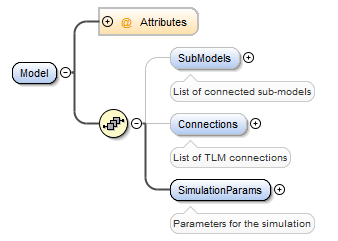
\includegraphics[width=\linewidth]{tlm_root_element.png}
	\caption{The Model (root) element of the Composite Model Schema.}
	\label{fig:tlmerootelement}
\end{figure}


The \textit{SimulationParams} element specify the start time and end time for the co-simulation.

The \textit{SubModel} element, presented in Figure \ref{fig:tlmsubmodelelement}, represents the simulation model component that participates in the co-simulation. The required attribute for a \textit{SubModel} are \textit{Name} of the sub-model, \textit{ModelFile} (file name of the submodel) and \textit{StartCommand} (the start method command to participate in the co-simulation). Each \textit{SubModel} also contains a list of interface points. \textit{InterfacePoint} elements are used to specify the \acrshort{tlm} interfaces of each simulation component (sub-model). 

\begin{figure}
	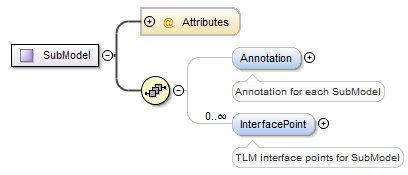
\includegraphics[width=\linewidth]{tlm_submodel_element.png}
	\caption{The SubModel element from the Composite Model Schema.}
	\label{fig:tlmsubmodelelement}
\end{figure}

The \textit{Connection} element of the composite model \acrshort{xml} schema is shown in Figure \ref{fig:tlmconnectionelement}.

\begin{figure}
	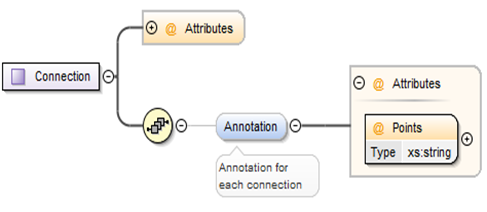
\includegraphics[width=\linewidth]{tlm_connection_element.png}
	\caption{The Connection element from the Composite Model Schema.}
	\label{fig:tlmconnectionelement}
\end{figure}

The \textit{Connection} element defines connections between two connected interface points, that is, 
a connection between two TLM interfaces. Its attributes \textit{From} and \textit{To} define which interface of which submodels are connected. Other attributes of the \textit{Connection} element specify the delay and maximum step size. 

\section{Composite Model Graphical Editor}
\label{sec:tlmeditor}

One of the primary contributions of this effort is our focus on interoperability in modeling and simulation.
Our effort leverage OpenModelica for graphical composite model editing as well as SKF’s co-simulation framework for TLM-based co-simulation. The implementation of this graphical composite model editor is an extension of OMEdit  which is implemented in C++ using the Qt graphical user interface library.

The full graphical functionality of the composite modeling process can be expressed in the following steps:

\begin{enumerate}
	
\item Import and add the external models to the composite model editor,
\item Specify startup methods and interfaces of the external model,
\item Build the composite models by connecting the external models,
\item Set the co-simulation and TLM parameters in the composite model.

\end{enumerate}

An overview of the different components that the graphical composite model editor relies on is shown in Figure \ref{fig:tlmeditorinteraction}. 

\begin{figure}
	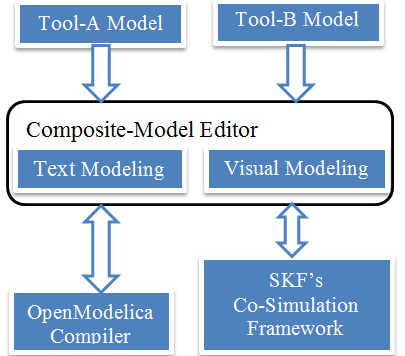
\includegraphics[width=\linewidth]{tlm_editor_interaction.png}
	\caption{An overview of the interaction between the composite model (meta-model) graphic editor and the other components.}
	\label{fig:tlmeditorinteraction}
\end{figure}

The graphical composite model editor communicates with the OpenModelica compiler to
retrieve the interface points for the external model and SKF’s co-simulation framework to run the \acrshort{tlm} simulation manager and simulation monitor. Each tool component is descried in the following subsections.

In the graphic composite model editor the modeling page area is used for visual composite modeling or text
composite modeling. This allows users to create, modify, and delete sub-models user-friendly. 

\subsection{Visual Modeling}
\label{sec:tlmvisual}

Each composite model has two views: a Text view and a Diagram view. In the diagram view, each simulation
model component (sub-model) of the \acrshort{tlm} cosimulation can be dragged and dropped from the library browser to this view, and then the sub-model will be automatically translated into a textual form by fetching the interface name for the \acrshort{tlm} based cosimulation. The user can complete the composite model (see Figure \ref{fig:tlmtest}) by graphically connecting components (sub-models).

\begin{landscape}
\begin{figure}
	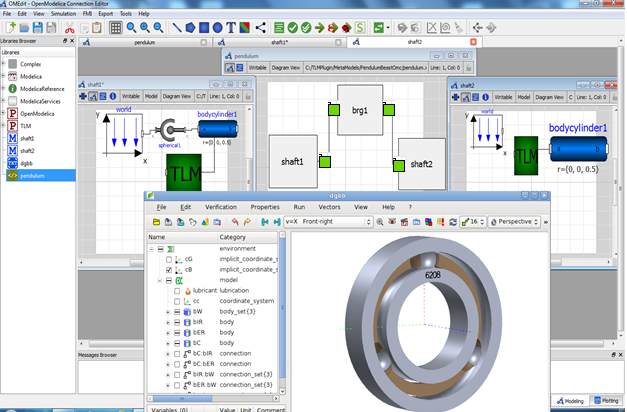
\includegraphics[width=\linewidth]{test_tlm.png}
	\caption{A screenshot of visual composite modeling of double pendulum.}
	\label{fig:tlmtest}
\end{figure}
\end{landscape}

The test model (see Figure \ref{fig:tlmtest} ) is a multibody system that consists of three sub-models: Two OpenModelica
\textit{Shaft} sub-models (\textit{Shaft1} and \textit{Shaft2}) and one SKF/BEAST bearing sub-model that together build a \textit{double pendulum}. The SKF/BEAST bearing submodel is a simplified model with only three balls to speed up the simulation. 

\textit{Shaft1} is connected with a spherical joint to the world coordinate system. The end of \textit{Shaft1} is connected via a \acrshort{tlm} interface to the outer ring of the BEAST bearing model. The inner ring of the bearing model is connected via another \acrshort{tlm} interface to \textit{Shaft2}. Together they build the double pendulum with two shafts, one spherical OpenModelica joint, and one BEAST bearing. 

\subsection{Textual Modeling and Viewing}
\label{sec:tlmtextual}

The text view (see Figure 8 \ref{fig:tlmtextview}) allows users to view the contents (sub-models, connections, and simulation
parameters) of any loaded composite model. It also enables users to edit a composite model textually as
part of the composite modeling construction process. To facilitate the process of textual composite modeling
and to provide users with a starting point, the text view (see Figure \ref{fig:tlmtextview}) includes the composite model \acrshort{xml}
schema elements and the default simulation parameters. 

\begin{landscape}
\begin{figure}
	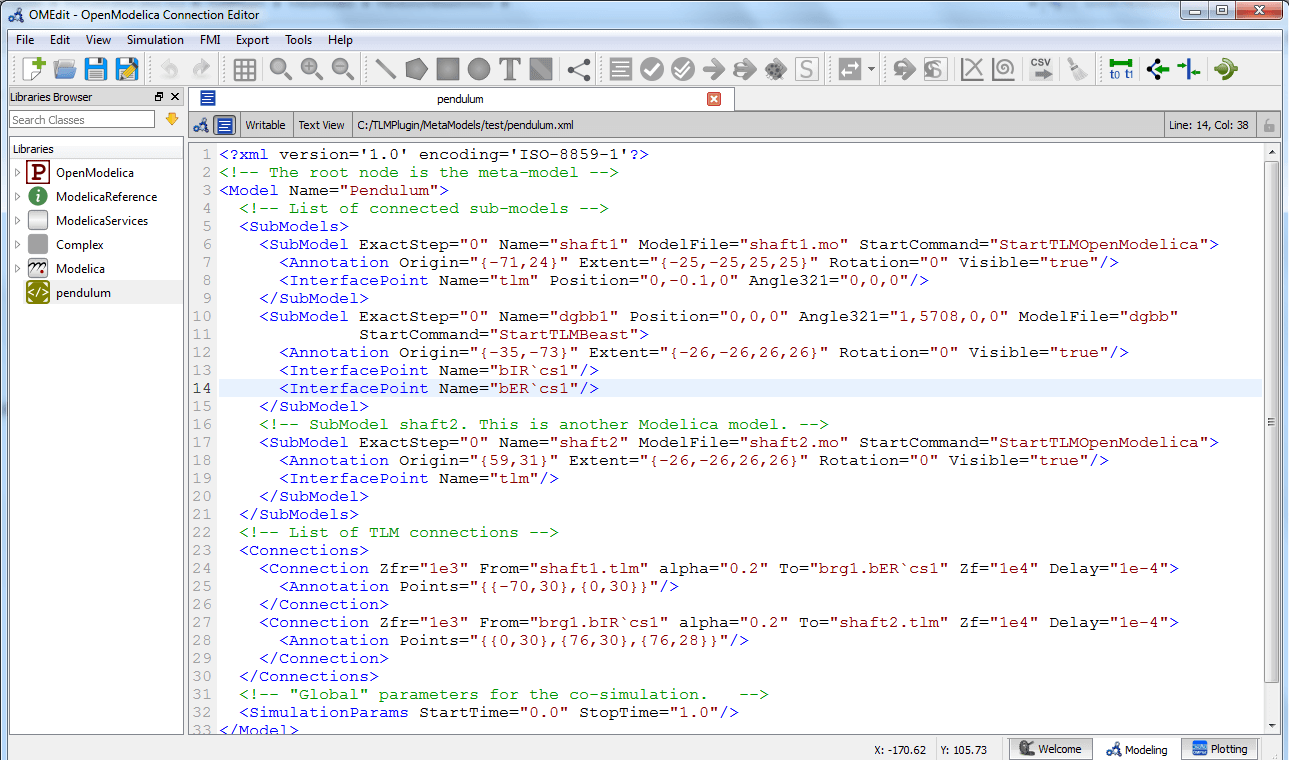
\includegraphics[width=\linewidth]{tlm_textview.png}
	\caption{A screenshot of textual composite modeling.}
	\label{fig:tlmtextview}
\end{figure}
\end{landscape}

\subsection{Composite Model Validation}
\label{sec:tlmvalidation}

Since model validation is part of the composite modeling process, the composite model editor supports users by validating the composite model to ensure that it follows the structure and content rules specified in the composite model schema described in Section 4. In general the composite model
editor validation mechanism supports users to verify that: 

\begin{itemize}

\item The basic structure of the elements and attributes in the composite model matches the composite model schema.
\item All information required by the composite model schema is present in the composite model.
\item The data conforms to the rules of the composite model schema.

\end{itemize}

\subsection{OpenModelica Runtime Enhancement}
\label{sec:tlmruntime}

To support \acrshort{tlm}-based co-simulation the OpenModelica runtime has been enhanced. The added
functionality supports single solver step simulation so that the executed simulation model can work together
with the \acrshort{tlm} manager. New flags to enable this functionality in the simulation executable are now available:

\begin{itemize}
		
\item -noEquidistantOutputFrequency
\item -noEquidistantOutputTime

\end{itemize}

The new flags control the output, e.g., the frequency of
steps and the time increment. 

\subsection{Communication with the SKF TLM Based Co-Simulation Framework}
\label{sec:tlmskf}

The graphic composite model editor in OpenModelica
provides a graphical user interface for co-simulation of
composite models. It can be launched by clicking the
\acrshort{tlm} co-simulation icon from the toolbar, see
Figure \ref{fig:tlmsetup}.

\begin{figure}
	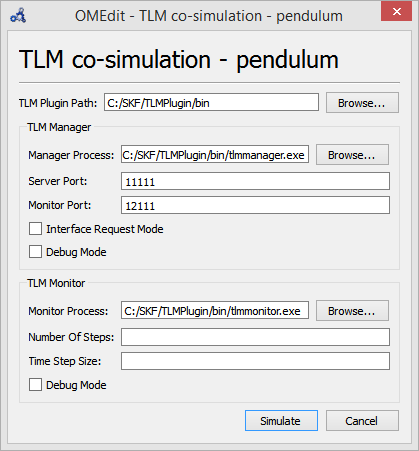
\includegraphics[width=\linewidth]{tlm_setup.png}
	\caption{TLM co-simulation setup.}
	\label{fig:tlmsetup}
\end{figure}

The editor runs the \acrshort{tlm} simulation manager and simulation monitor. The simulation manager reads the
composite model from the editor, starts the cosimulation, and provides the communication bridge
between the running simulations. Figure \ref{fig:tlmcosimulationprogress} shows the running status of the \acrshort{tlm} co-simulation.

\begin{figure}
	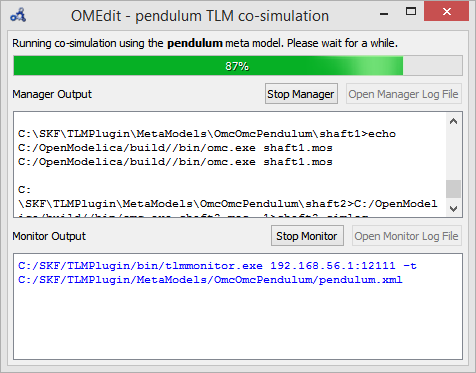
\includegraphics[width=\linewidth]{tlm_cosimulation_progress.png}
	\caption{TLM co-simulation.}
	\label{fig:tlmcosimulationprogress}
\end{figure}

The simulation monitor communicates with the simulation manager and writes the status and progress of the co-simulation in a file. This file is read by the editor for showing the co-simulation progress bar to the user. The editor also provides the means of reading the log files generated by the simulation manager and monitor.

During the post-processing stage, simulation results are collected and visualized in the OMEdit 
plotting perspective as shown in Figure \ref{fig:tlmsimulationresults}.
 
\begin{figure}
	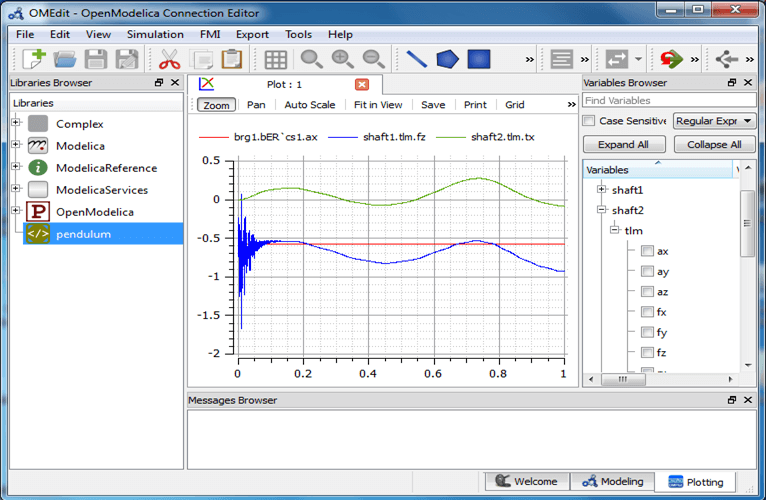
\includegraphics[width=\linewidth]{tlm_simulation_results.png}
	\caption{Results of TLM co-simulation.}
	\label{fig:tlmsimulationresults}
\end{figure}


\subsection{Industrial Application of Composite Modeling with TLM Co-Simulation}
\label{sec:tlmapplication}

SKF has successfully used the \acrshort{tlm} co-simulation framework to simulate composite models. For
example, Figure \ref{fig:tlmapplication} shows one such application with an MSC.ADAMS \cite{adams} car model
containing an integrated SKF BEAST\cite{beast} hub-unit sub-model 
connected via \acrshort{tlm}-connections.

\begin{figure}
	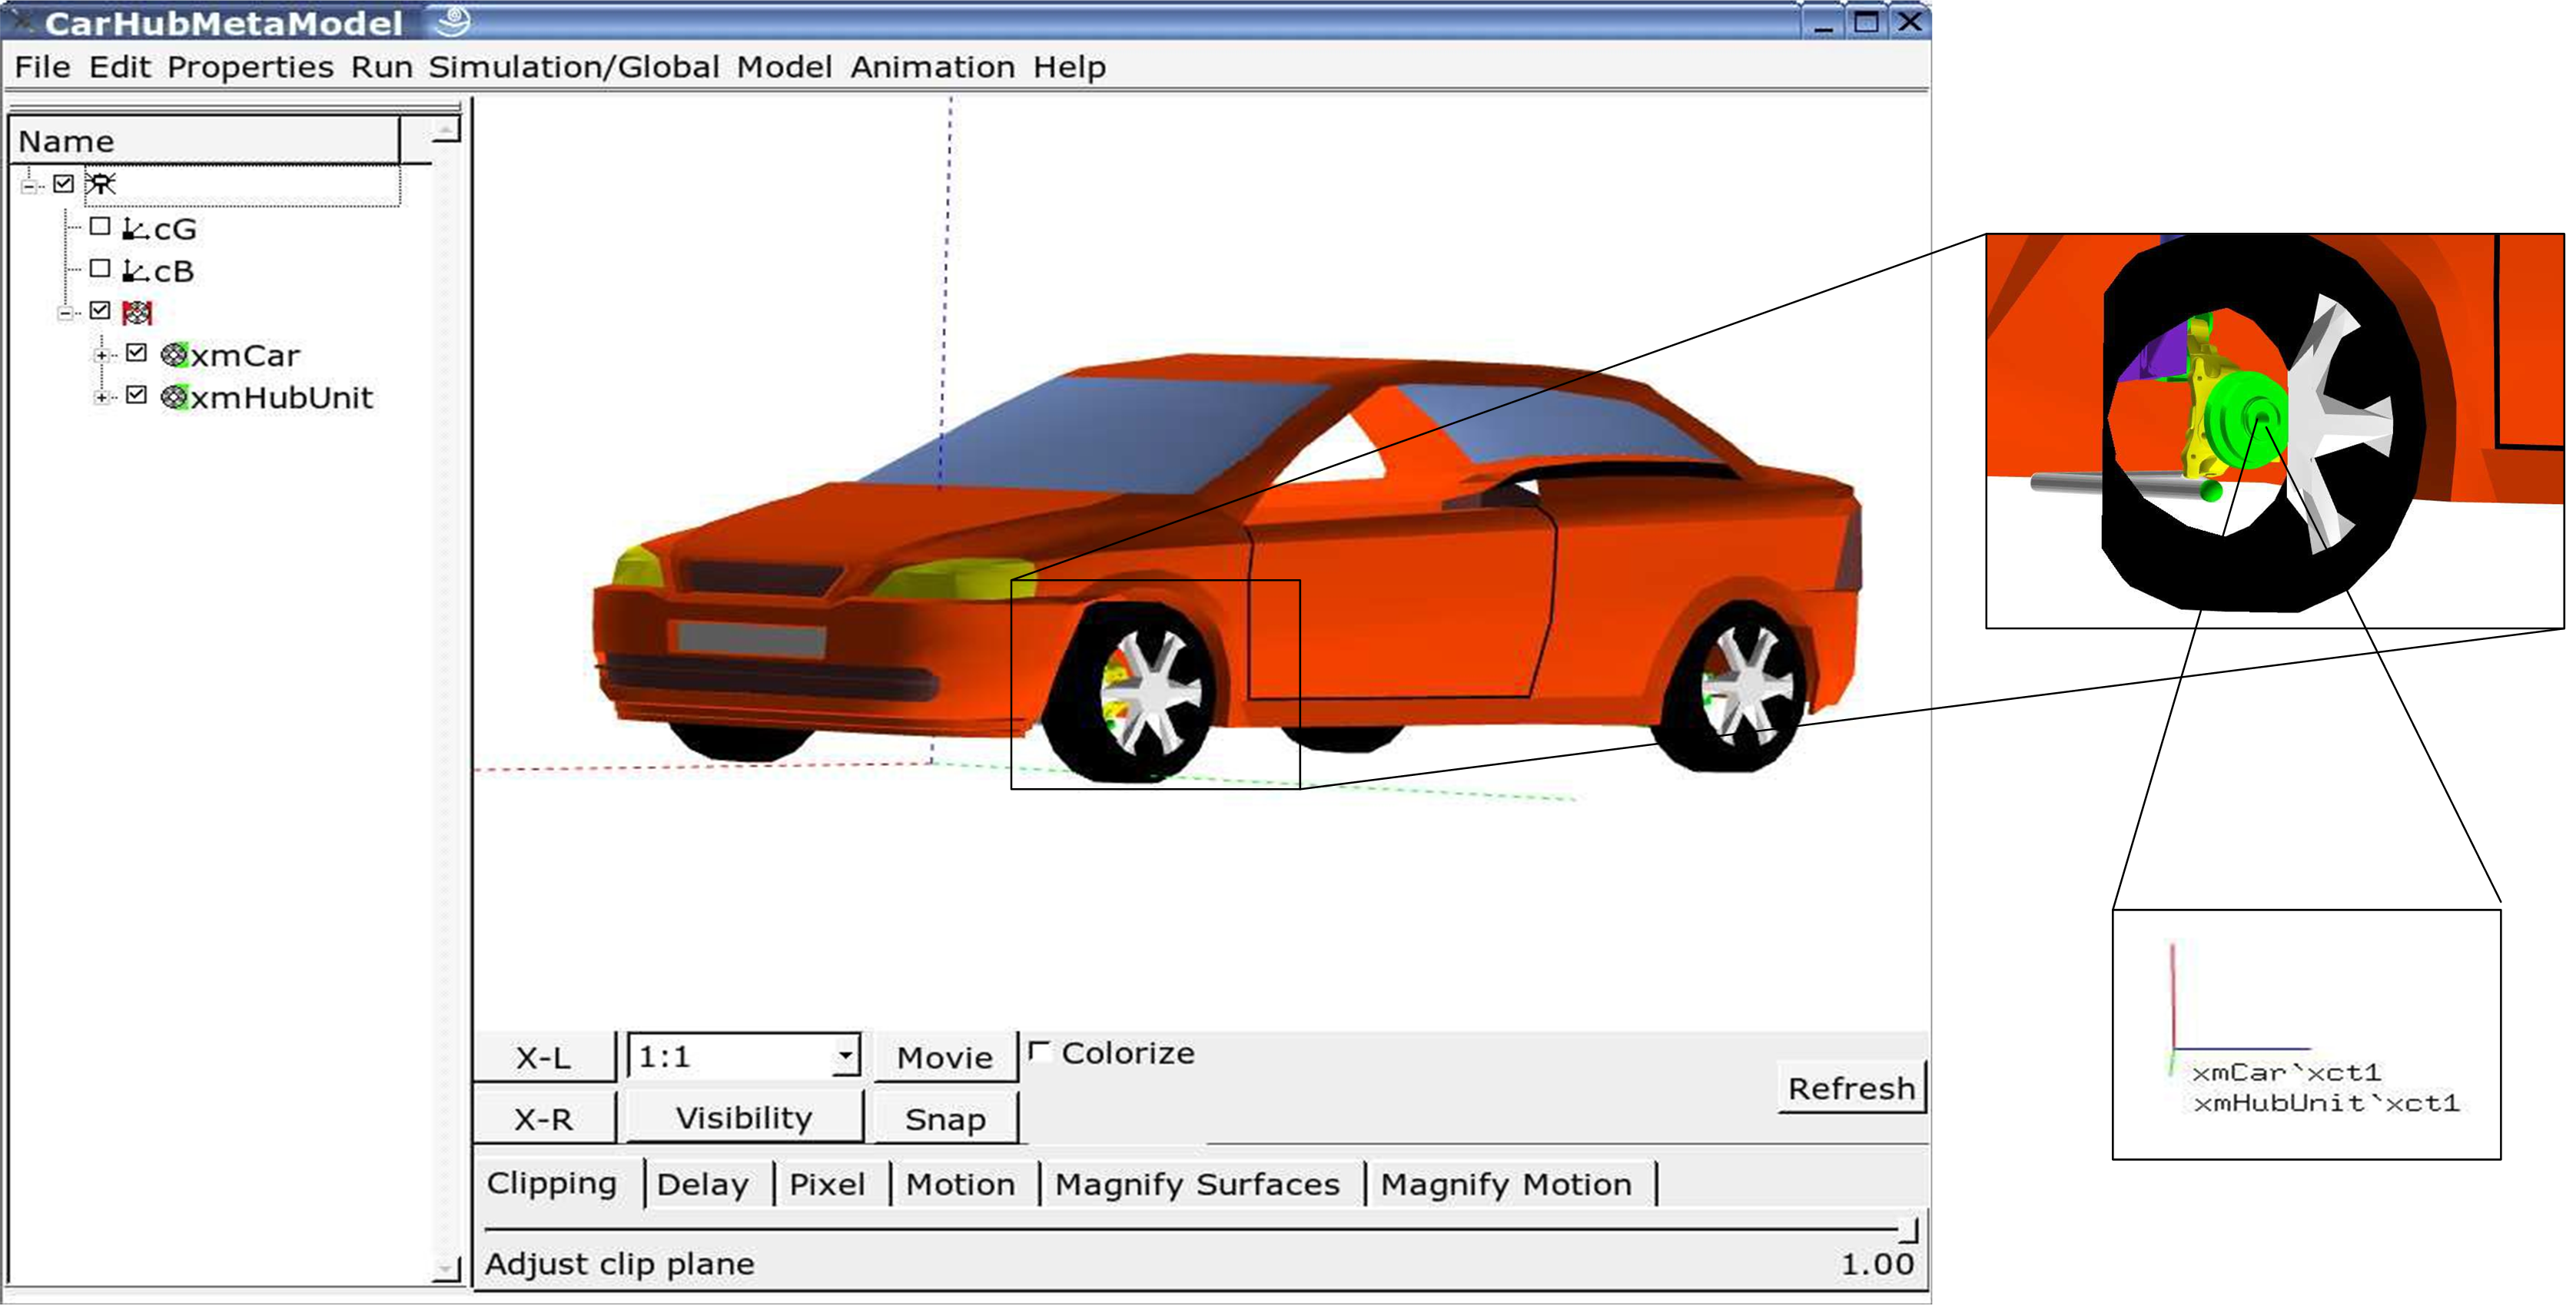
\includegraphics[width=\linewidth]{tlm_application.png}
	\caption{A composite model of an MSC.ADAMS car model with an integrated SKF BEAST hub-unit sub-model (green), connected 
		     via TLM connections for co-simulation.}
	\label{fig:tlmapplication}
\end{figure}

\section{Summary}
\label{sec:tlmsummary}

In this chapter, we introduced a general open-source graphical editor and simulation tool for composite modeling and co-simulation as well as its integration with SKF’s TLM-based co-simulation framework for TLM based co-simulation. The graphical editor combines a number of features to support end-users with respect to the creation of composite models and co-simulation. These include adding, removing, and connecting components (submodels) both textually and graphically, as well as integrated co-simulation and visualization of simulation results. The composite model editor supports external non-Modelica models represented in XML form (essentially black boxes with interfaces) inside the component tree which can be used for composite model composition. A number of tool specific simulation models, such as Modelica models, SimuLink models, Adams models, BEAST models,
etc., have successfully been connected and simulated using TLM based co-simulation. A schema for validation of a composite modeling has been developed as a part of this work. 

\subsection*{Acknowledgements}
\label{sec:tlmAcknowledgements}

The work has been supported by Vinnova in the ITEA2
MODRIO project, by EU in the INTO-CPS project, and by the Swedish Government in the Swedish
Government in the ELLIIT project. The open-source Modelica Consortium supports the OpenModelica
work. The TLM based co-simulation framework is provided by SKF.


%\nocite{scigen}
%We have included Paper \ref{art:scigen}

%%%%%%%%%%%%%%%%%%%%%%%%%%%%%%%%%%%%%%%%%%%%%%%%%%%%%%%%%%%%%%%%%%%%%%
%%% Intro.tex ends here


%%% Local Variables: 
%%% mode: latex
%%% TeX-master: "demothesis"
%%% End: 
